\documentclass{beamer}

\usepackage{beamerthemesplit}
\usepackage{wasysym}
\usepackage{amsmath, mathtools}
\usetheme{Berlin}

\title{MR-HIFU}
 \author{ \textcolor{red}{Rob Andrews, Chris Budd, Jessica Cervi, Joseph Feribach, Jim Keener, Jonathan Murley, Siv Sivaloganathan, Jeremy Tan}}
\date{\today}


\begin{document}
\begin{frame}
\maketitle
\end{frame}
\begin{frame}
 \tableofcontents
\end{frame}

\section{The Problem}
\subsection{Background}
\begin{frame}
\frametitle{The MR-HIFU Process}

HIFU is a process which may be used in destroying cancerous tissue using \textcolor{red}{hyperthermia}

\vspace{0.25in}

\begin{itemize}
\item Transducer produces \textcolor{purple}{40W Ultrasound signal at 1.2 MHz.}
\item Ultrasound signal is focused into a region $8mm \times 2mm \times 2mm$.
\item Pressure variations due to the ultrasound lead to a temperature source \textcolor{red}{$Q({\mathbf x},t)$.}
\item Temperature \textcolor{red}{$T(x,t)$} changes due to the action of the source, \textcolor{blue}{diffusion} and \textcolor{orange}{perfusion} due to blood flow.
\item High temperatures over a sustained time lead to \textcolor{red}{tissue damage.}
\end{itemize}



\end{frame}


\begin{frame}
\frametitle{}
\begin{center}
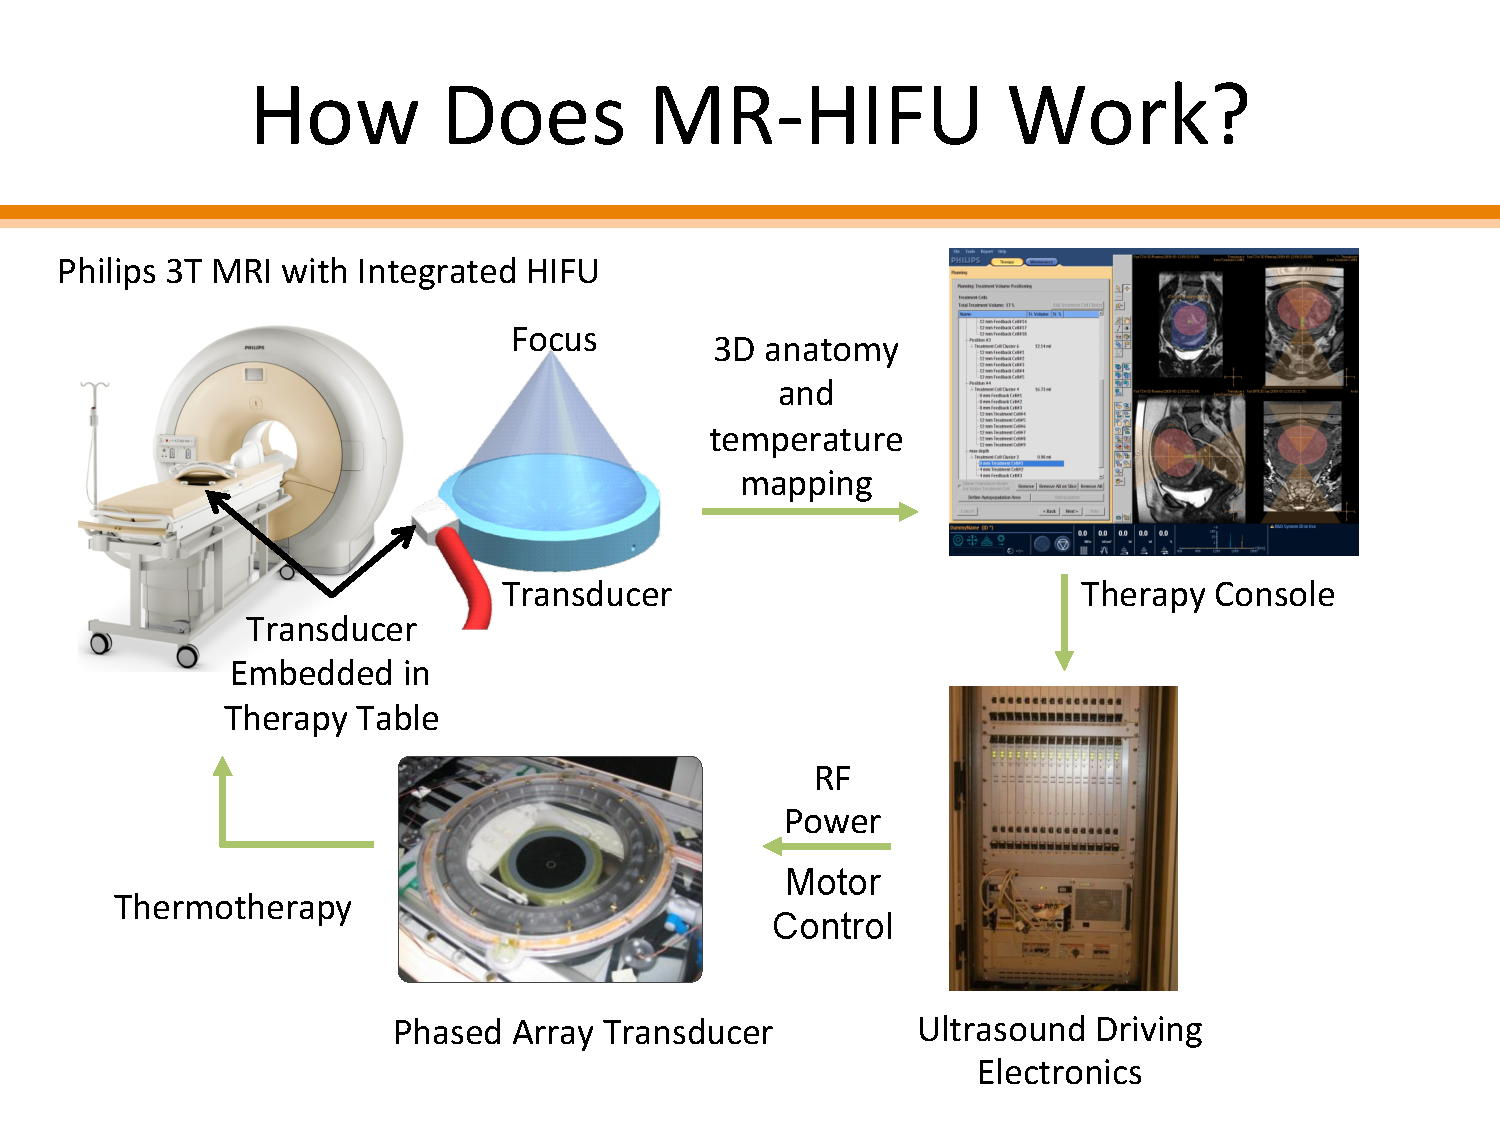
\includegraphics[scale=0.4]{Pages/MR-HIFU11a.pdf}
\end{center}
\end{frame}
\begin{frame}
\frametitle{}
\begin{center}
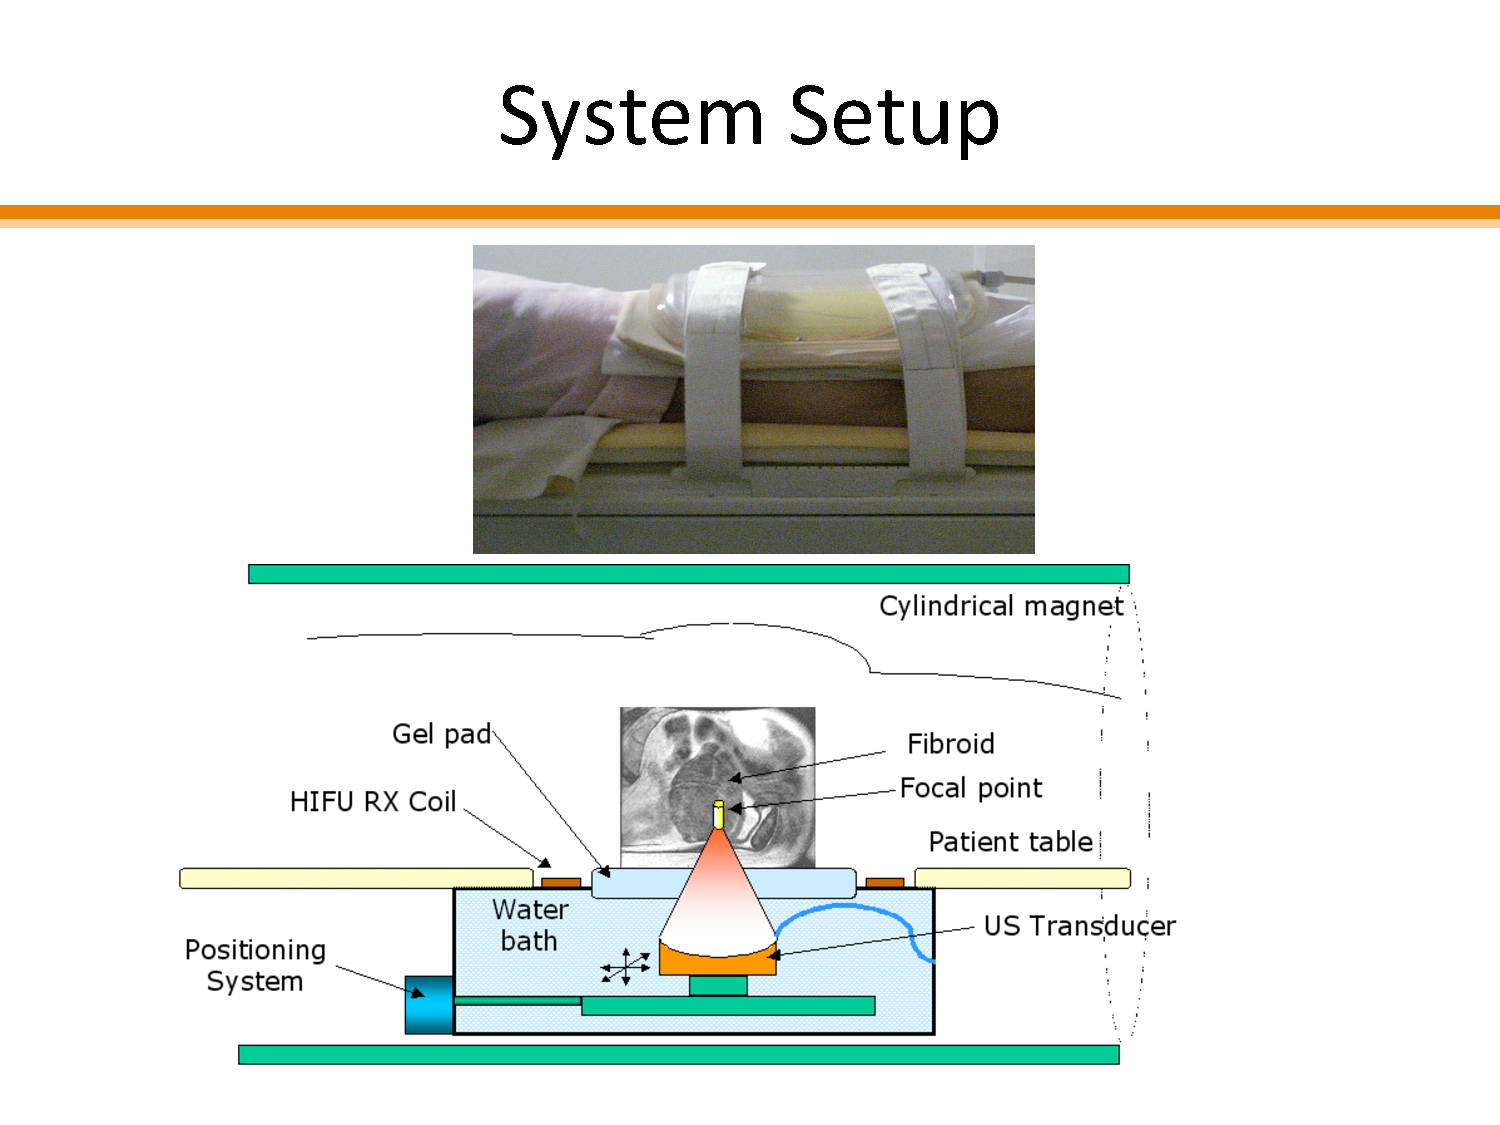
\includegraphics[scale=0.4]{Pages/MR-HIFU12a.pdf}
\end{center}
\end{frame}


\subsection{Questions}
\begin{frame}
\frametitle{Questions to address}
\begin{itemize}
\item Find a semi-analytic expression for the \textcolor{red}{spatially extended temperature field $T(x,t)$}
\item Obtain numerical computations of a \textcolor{blue}{simplified model} which allows us to look at the \textcolor{purple}{effects of parameter variation} and compare these with calculations from a more sophisticated model
\item Determine \textcolor{red}{useful and usable models for the spatial  tissue damage} which depend on material parameters which  takes
into
account
the
thermal
dose,
thermal
conductivity,
thermal
diffusion,
specific
heat,
and
perfusion
of
the
issue
of
interest
and
surrounding
structures.
\end{itemize}
\end{frame}



\section{Basic Physics}
\subsection{The source term $Q$}
\begin{frame}
\frametitle{The source term $Q$}

\begin{itemize}

\item Transducer produces a pressure field $P$ computable using a Rayleigh-Sommerfeld integral method.

\item This gives a heat source $Q$ with
$$\textcolor{orange} {Q = \frac{ \alpha P^2}{2 \rho c}.}$$
\end{itemize}

\end{frame}

\begin{frame}
\frametitle{Orthogonal components of pressure}

$P$ \textcolor{purple}{along} axis of propagation
$$ |P| = Ae^{-\alpha z} \big|1-e^{i k a^2/2z}\big| $$
$P$ \textcolor{orange}{orthogonal} to axis of propagation
$$ |P| = \frac{J_1(ky)}{ky} $$

\begin{center}
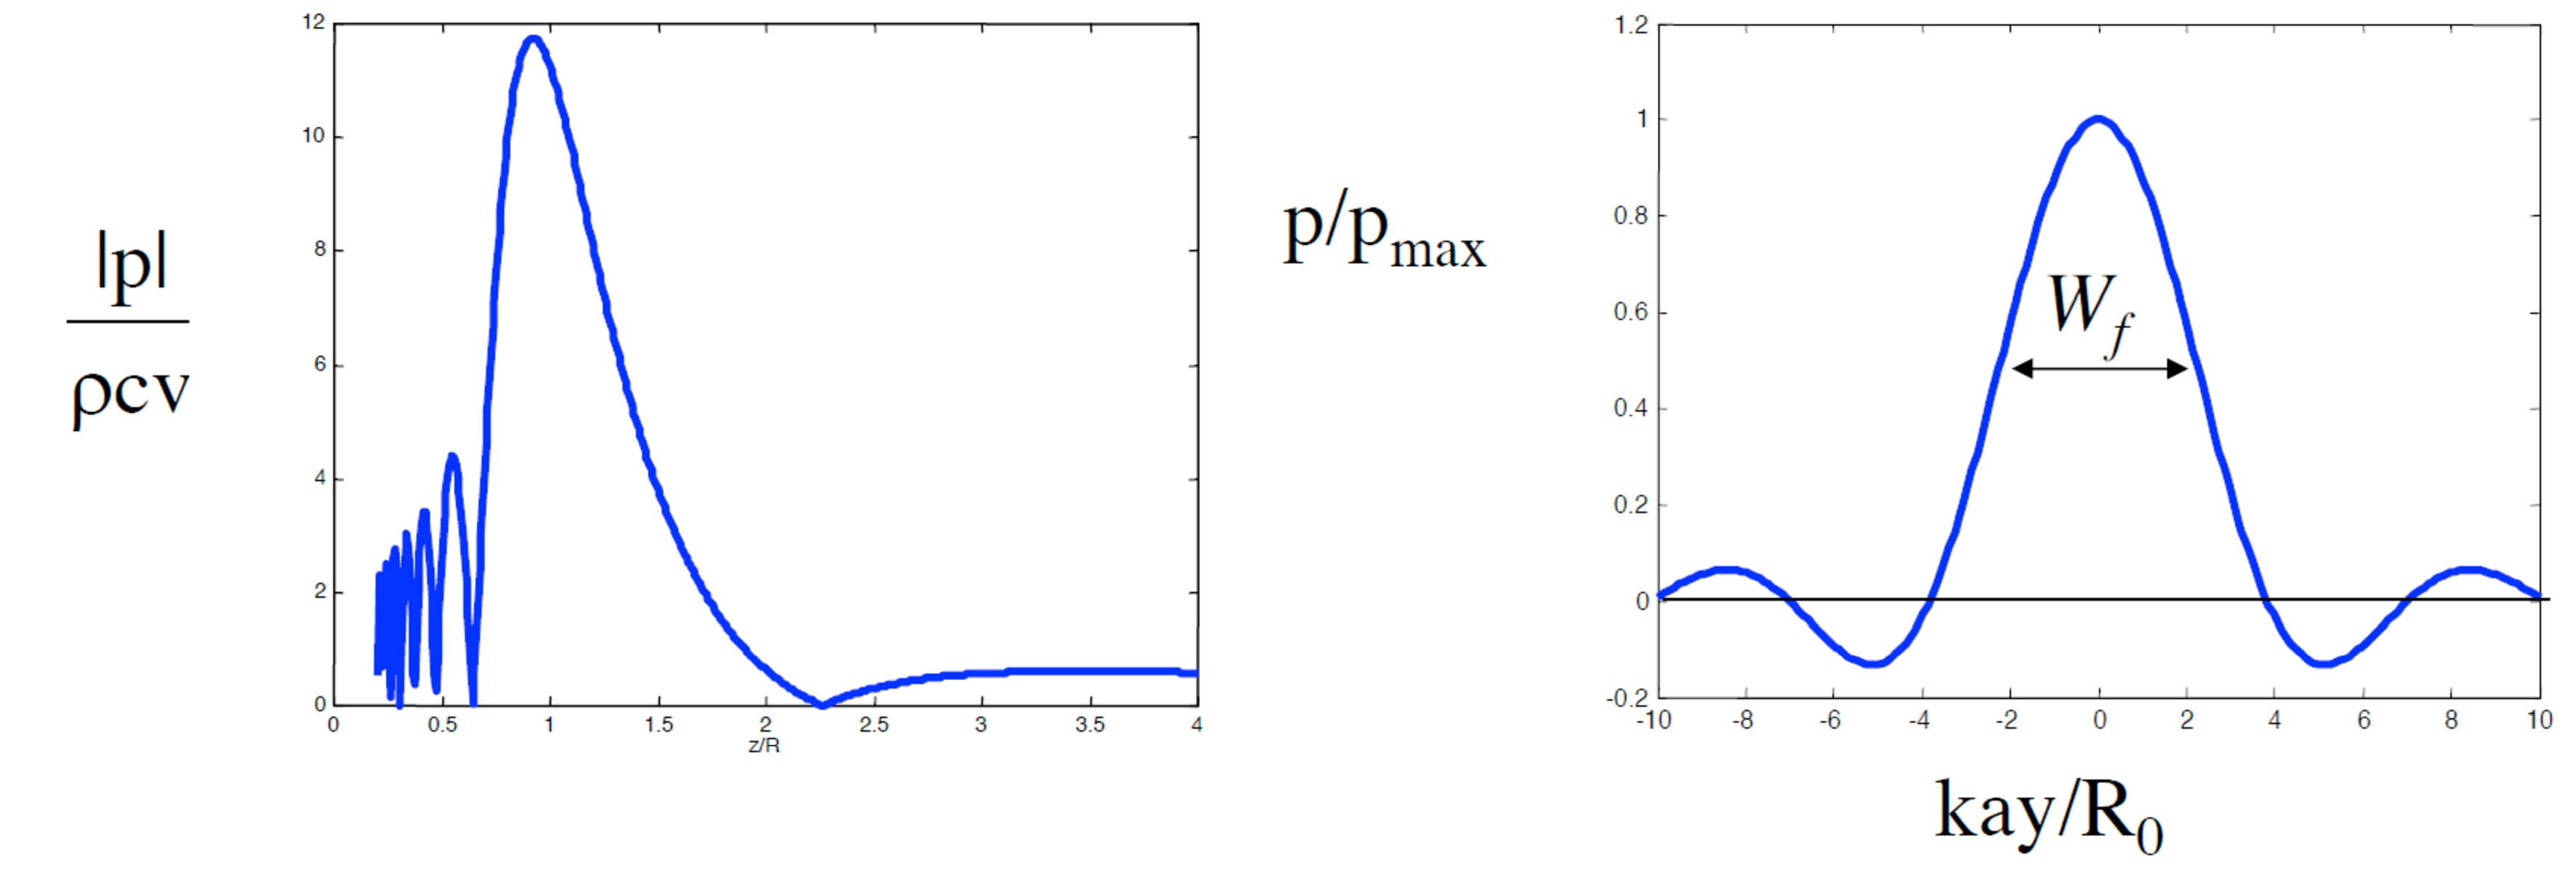
\includegraphics[scale=0.15]{Pages/transducer2731.pdf}
\end{center}

\end{frame}


\subsection{Pennes equation}
\begin{frame}
\frametitle{Pennes Equation}

The temperature $T(x,t)$ obeys the \textcolor{blue}{Pennes equation}: a \textcolor{purple}{linear heat equation}.

\textcolor{red}{Heat generation} due to source $Q$, \textcolor{blue}{Heat loss} due to conduction and perfusion by blood

$$\rho c T_t = \textcolor{blue}{\nabla (k \nabla T) - \gamma (T- T_b)} +\textcolor{red} Q.$$


$k$ is \textcolor{blue}{thermal conductivity} , $\gamma$ is the \textcolor{orange}{perfusion constant} (material dependent).Some values:

\begin{itemize}
\item $\rho c \approx 3 \times 10^6$
\item $\gamma \approx 2000$
\item $ Q \approx 4\rho c -10 \rho c $
\item Length scale of $L \approx 10^{-3}$ at the focus.
\item$k \approx 1/2$
\end{itemize}

\end{frame}

\subsection{Scalings}
\begin{frame} 
\frametitle{Some scalings}

\begin{itemize}

\item At the \textcolor{red}{ focus} 
$$\nabla (k \nabla T) \approx 10^6,  \gamma (T- T_b) \approx 10^3, Q \approx 10^6$$
Perfusion is unimportant (unless we are close to a major blood vessel).

\item Away from the focus, $Q$ diminishes rapidy (inverse square) and both perfusion and diffusion act together to reduce the temperature.

\end{itemize}


\end{frame}

\section{Simple Models}
\begin{frame}
\frametitle{Simple models}
Semi-analytic model of a \textcolor{red}{radially symmetric system}  \textcolor{blue}{close to the focus}.  

Let $r$ be the \textcolor{red}{distance from the focus}. Length scale \textcolor{blue}{$L = 10^{-3}$}

Set \textcolor{red}{$s = r/L$}. Use approximation
\textcolor{purple}
{
$$Q = Q_0 \rho c \left( \frac{J_1(r/L)}{r/L} \right)^2 = Q_0 \rho c \left( \frac{J_1(s)}{s} \right)^2.$$
}

Rescale system with known parameter values to give

$$\textcolor{blue}{T_t = \frac{1}{6s}  (s T)_{ss} - \frac{2}{3} \times 10^{-3} (T-T_b) + Q_0 \left( \frac{J_1(s)}{s} \right)^2} $$
\textcolor{red}{$$T_s(0) = 0, \quad T(\infty) = T_b.$$}
\end{frame}

\begin{frame}
\frametitle{Numerical calculation}
\begin{itemize}

\item Solve this numerically with a \textcolor{red}{Crank-Nicolson method}
$$\Delta t = 1, \Delta x = 0.04, x \in [0,20].$$

\item Test by using \textcolor{purple}{$Q = \sin(r)/r$} which gives an \textcolor{orange}{analytic solution}.

\item Method converges rapidly using sparse matrix methods

\item Run with $Q$ as before with \textcolor{red}{$Q_0 = 5$} for $0 < t < 30s$. 

\item Then take \textcolor{blue}{$Q_0 = 0$} for $t > 30$.

\end{itemize}

\end{frame}

\begin{frame}
\frametitle{Results}
\begin{center}
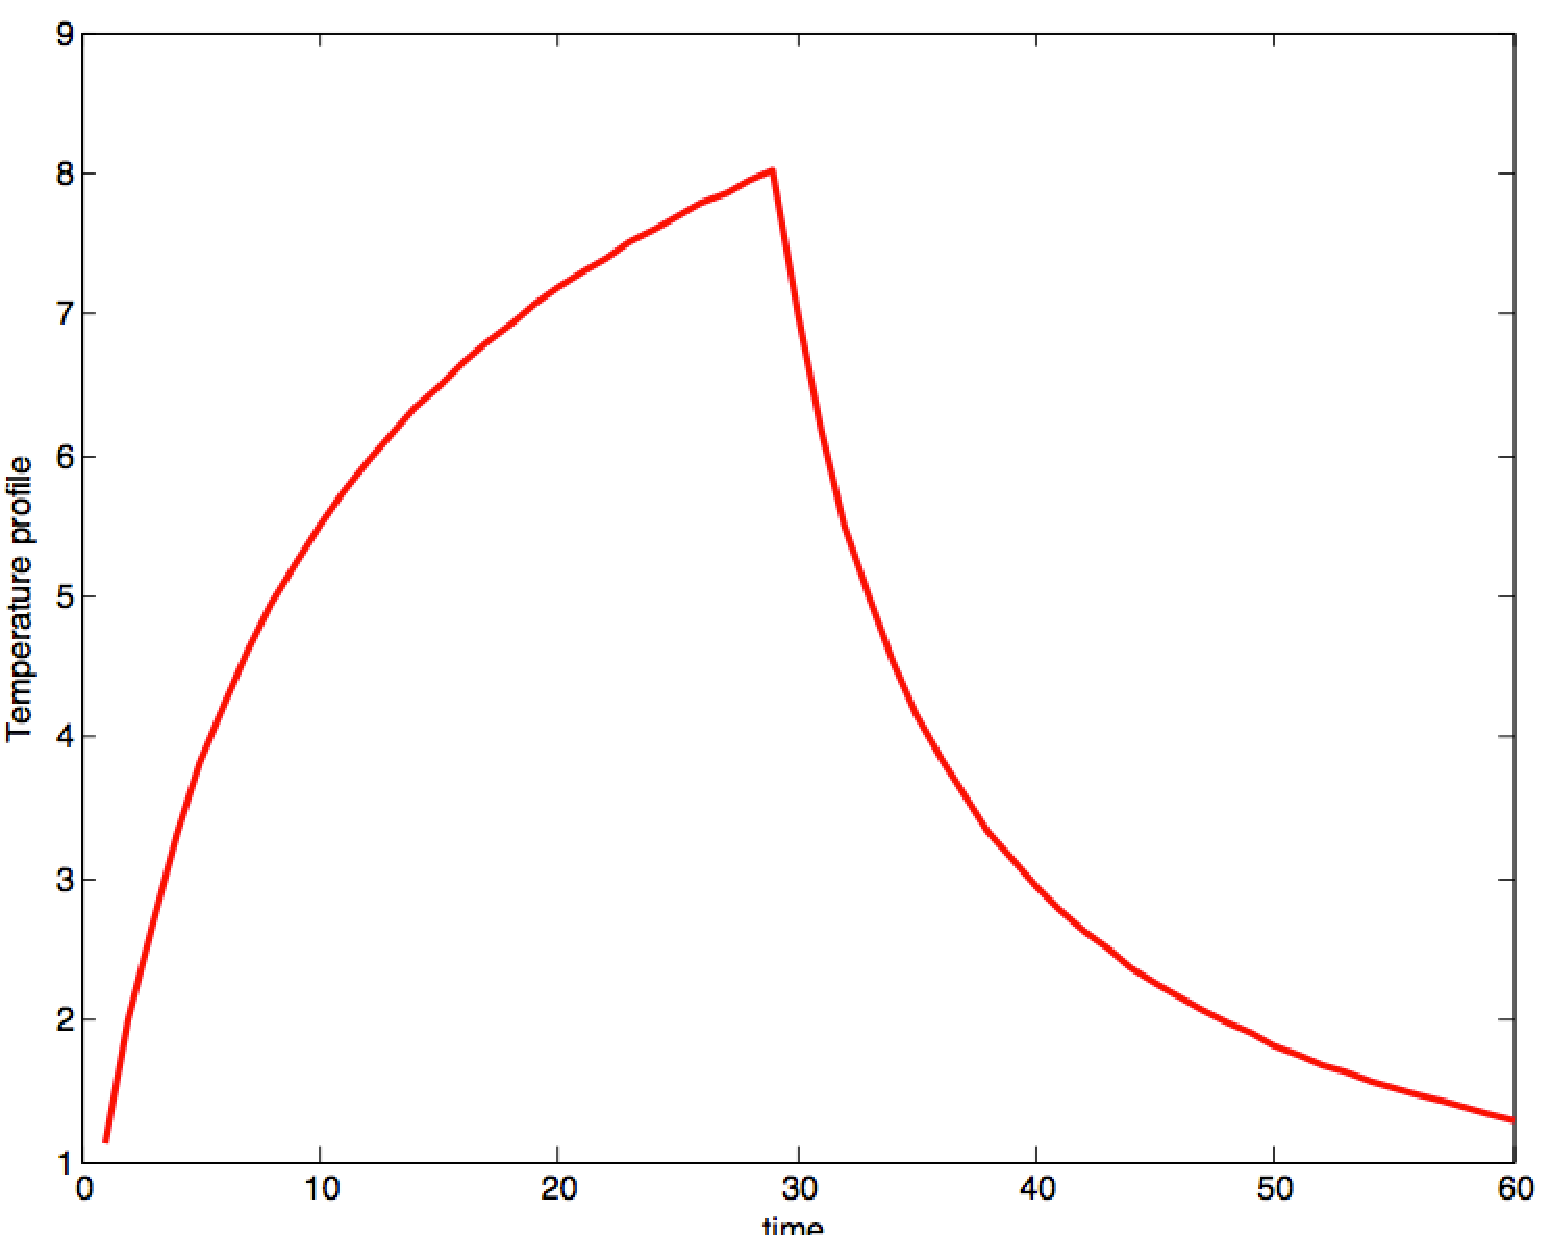
\includegraphics[scale = 0.42 ]{Pages/Temperature_profile_Jessica.pdf}
\end{center}
\end{frame}
\begin{frame}
\frametitle{Results}
\begin{center}
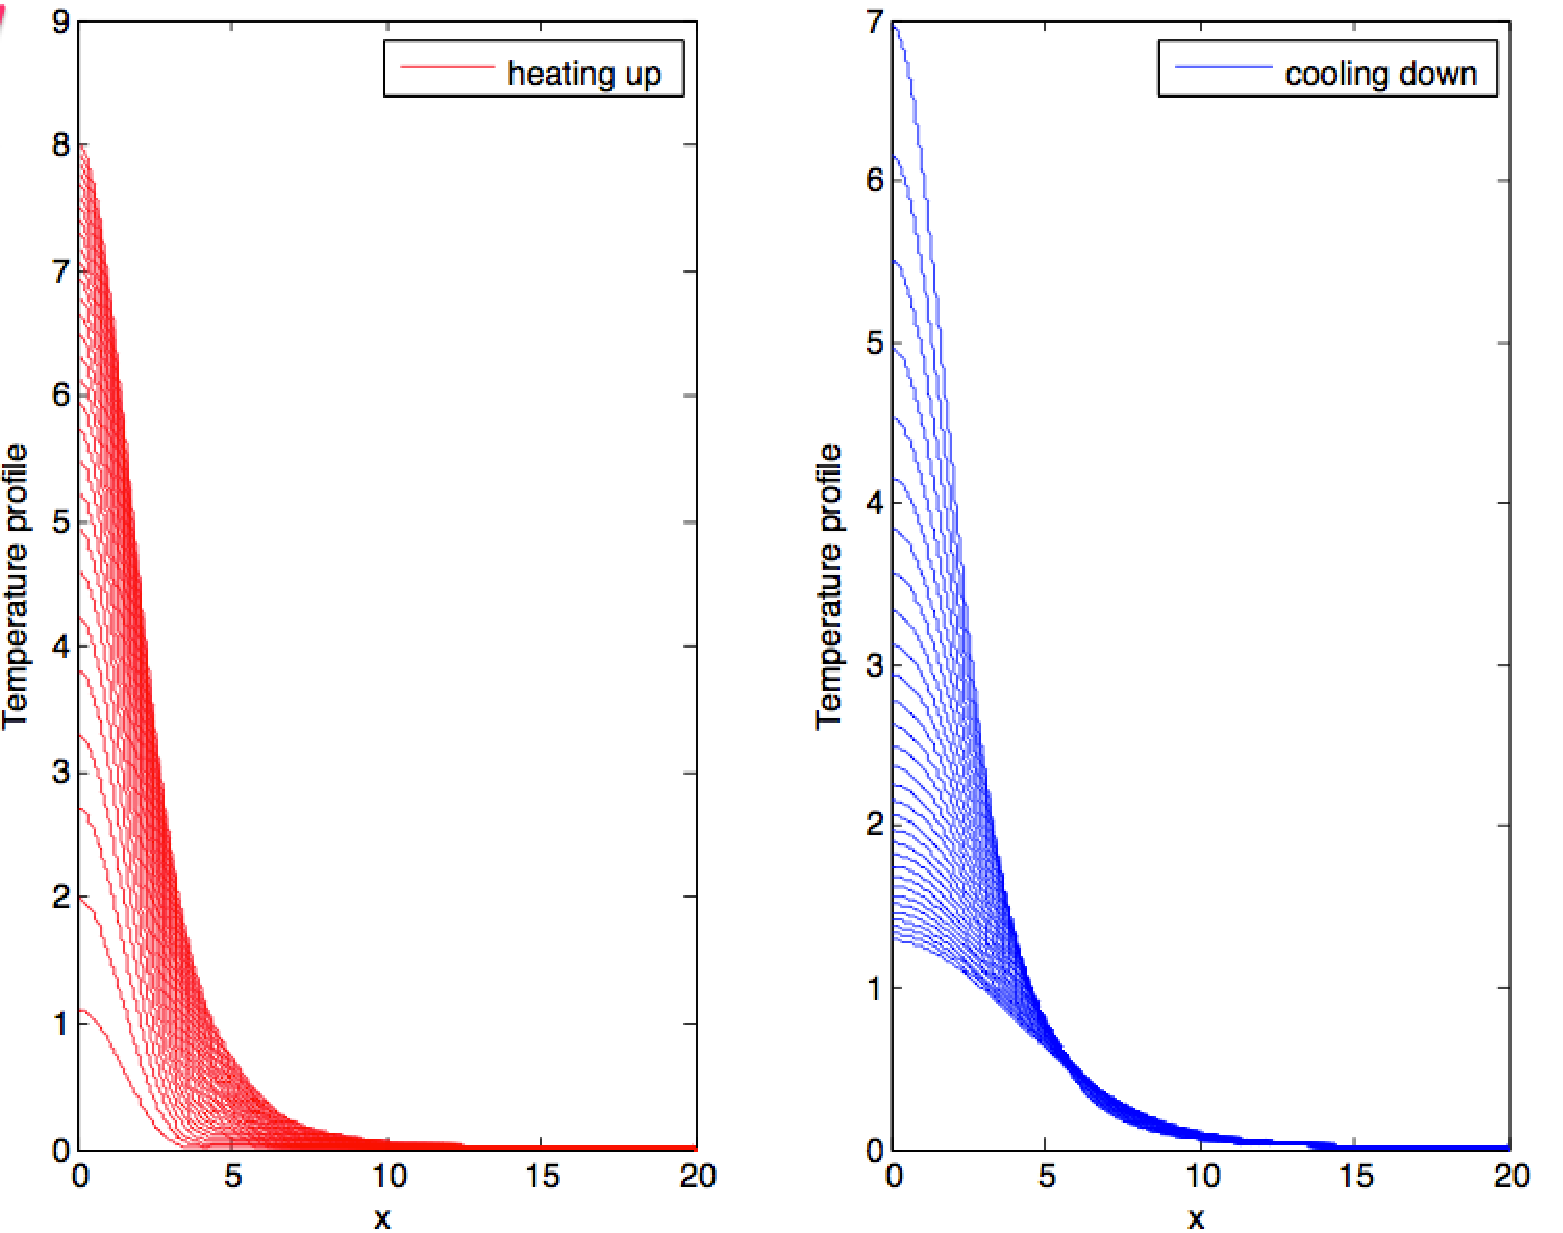
\includegraphics[scale = 0.3]{Pages/heating_cooling_Jessica.pdf}
\end{center}
\end{frame}

\begin{frame}
\frametitle{Comparison with results from more complex (3D finite difference) models}
\begin{center}
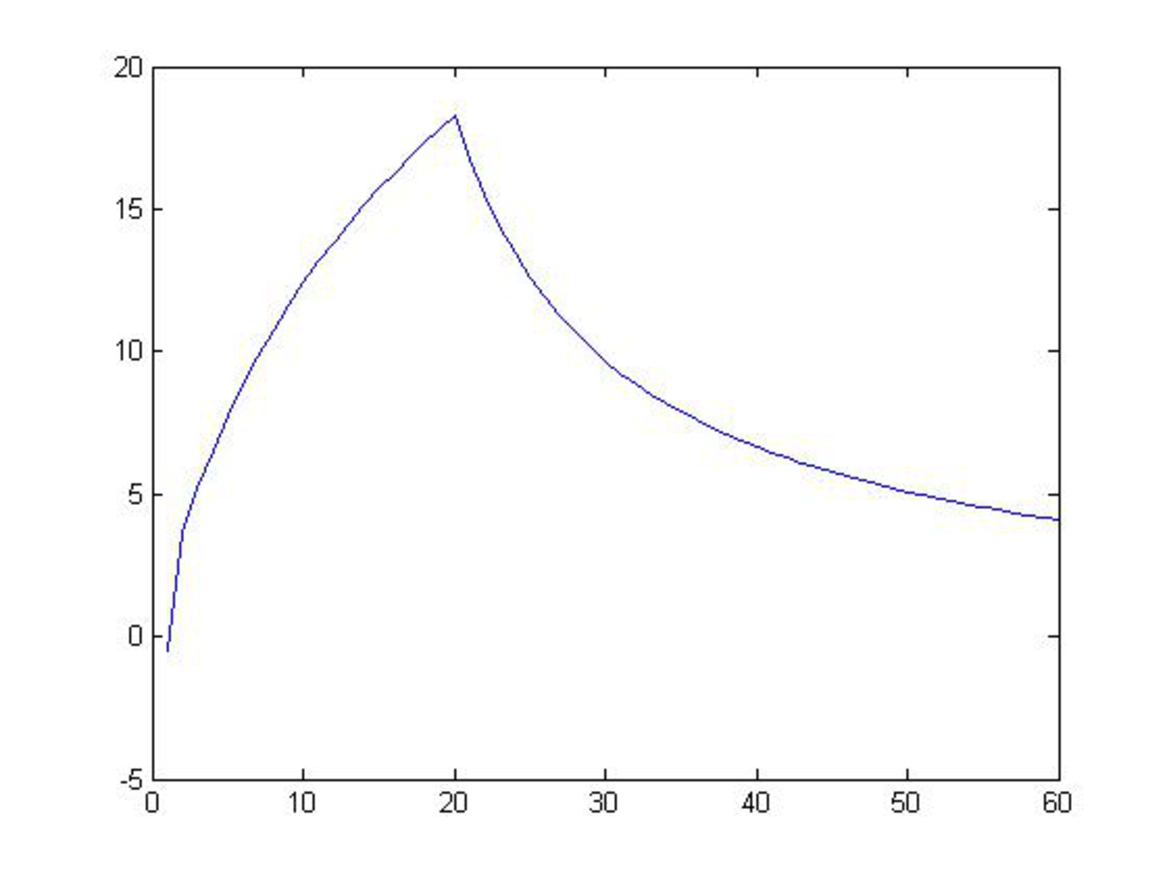
\includegraphics[scale=0.4]{Pages/jmurleymaxtemp.pdf}
\end{center}
\end{frame}
\begin{frame}
\frametitle{Comparison with results from more complex (3D finite difference) models}
\begin{center}
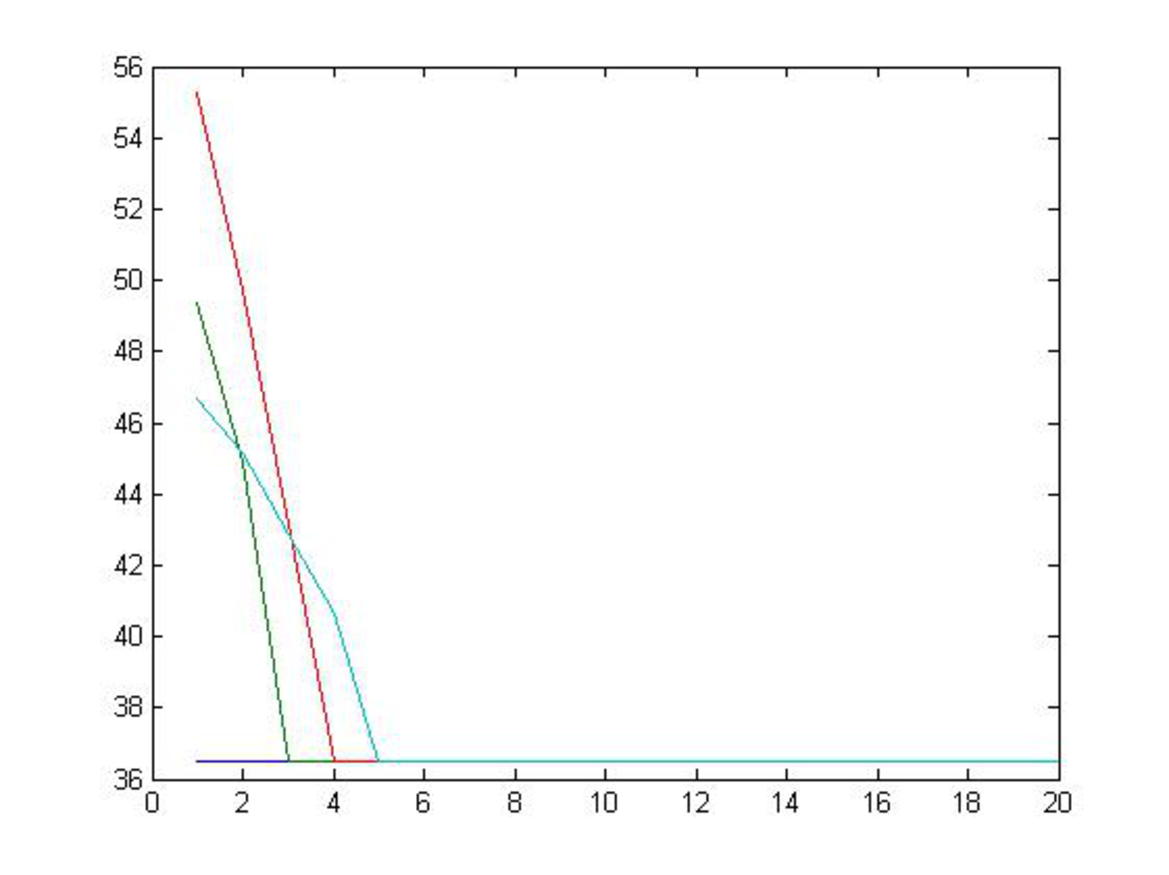
\includegraphics[scale=0.4]{Pages/jmurleytemprising.pdf}
\end{center}
\end{frame}
\begin{frame}
\frametitle{Comparison with results from more complex (3D finite difference) models}
\begin{center}
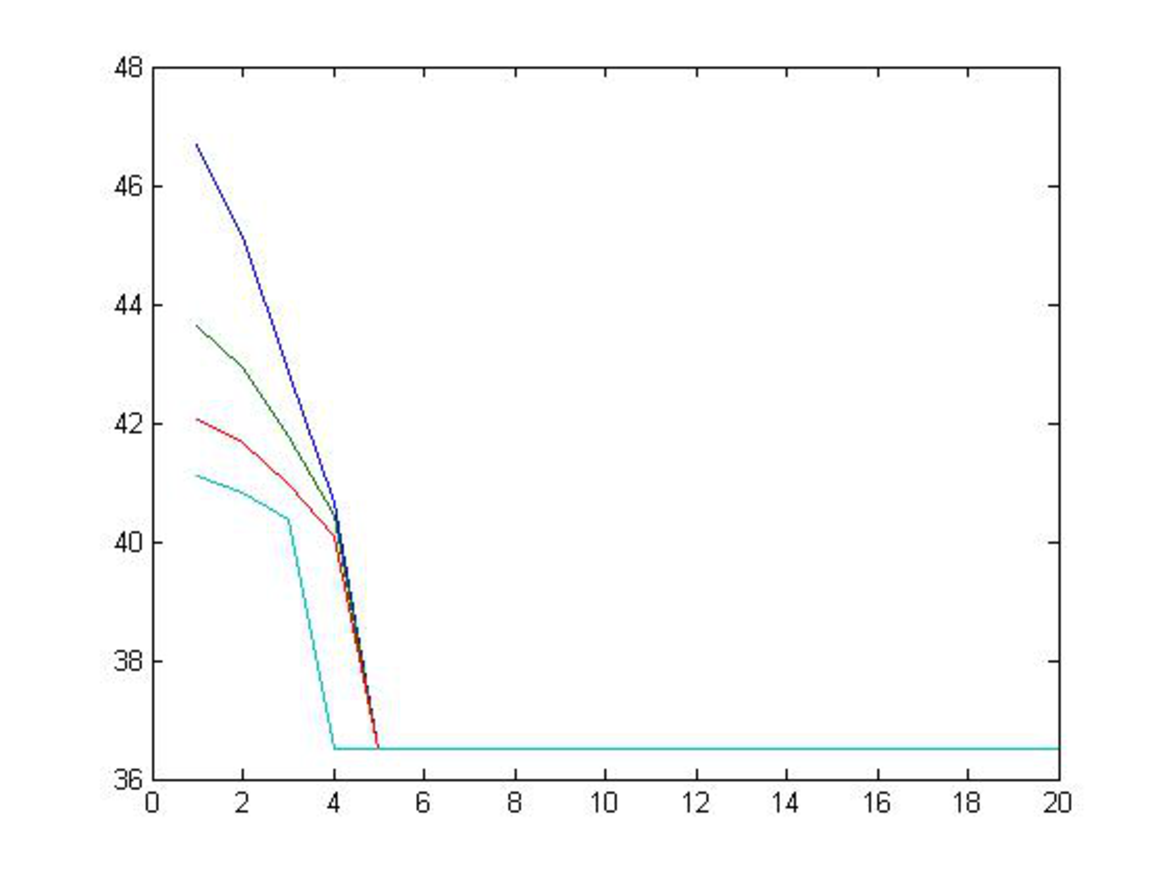
\includegraphics[scale=0.4]{Pages/jmurleytempfalling.pdf}
\end{center}
\end{frame}
\begin{frame}
\frametitle{Comparison with results from more complex (3D finite difference) models}
\begin{center}
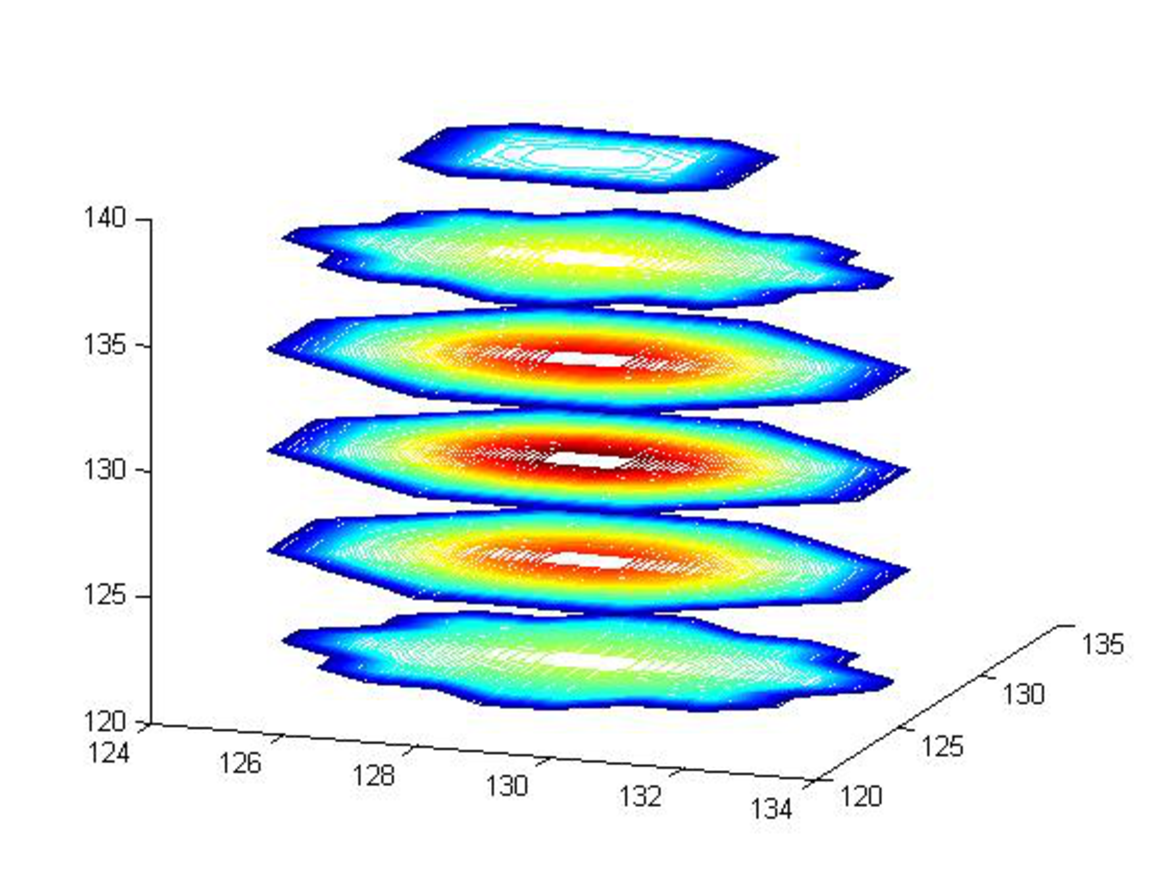
\includegraphics[scale=0.4]{Pages/jmurleycontourslices.pdf}
\end{center}
\end{frame}


\section{Damage Theory}
\subsection{Background}
\begin{frame}
\frametitle{Classical DamageTheory}
Classical theory (widely accepted, \textcolor{blue}{Saparto and Dewey, 1984}) is based on the assumption that damage  is measured by 
\begin{equation*}
\textcolor{blue}{TD(t) = \int_0^tr^{(43-T(t))}dt}\qquad r = \left\{\begin{array}{cc}0.25 & T\le43^oC\\0.50&T>43^oC\end{array}\right.
\end{equation*}

This formula 
\begin{itemize}
\item is \textcolor{red}{entirely phenomenological/heuristic} (has no mechanistic basis);
\item Damage threshold \textcolor{red}{varies widely} among different tissues;
\item No explanation of the significance/origin of the threshold at 43$^o$C.
\end{itemize}



\end{frame}

\begin{frame}
\frametitle{Another Idea}
\textcolor{blue}{Zhou, Chen, and  Zhang, 2007} suggested that damage is the result of \textcolor{orange}{irreversible, protein denaturization}, governed by the chemical reaction
\begin{equation*}
P\rightarrow D,
\end{equation*}
($P =$ folded protein, $D=$ denatured protein) at an \textcolor{red}{Arrhenius reaction rate}
\begin{equation*}
\textcolor{orange}{r(T) = A\exp\left(-\frac{\Delta G}{RT}\right)}
\end{equation*}
where $\Delta G$ is activation energy, $R$ is universal gas constant.

This leads to damage fraction
\textcolor{red}
{
\begin{equation*}
\Omega(t) = \log\left(\frac{P_0}{P(t)}\right) = \int_0^tA\exp\left(-\frac{\Delta G}{RT(t)}\right) \; dt
\end{equation*}
}
($P_0=$ initial folded protein).
 
\end{frame}
 

\begin{frame}
\frametitle{Comments}
\begin{itemize}
\item While this formula was used for damage from a laser, we believe it is also applicable to damage from ultrasound (HIFU);
\item The parameters $A$, $\Delta G$ and $\Omega_\theta$ (damage threshold) can be \textcolor{red}{chosen to match different tissue types.}
\item $\Omega(t)$ can be readily computed using the \textcolor{blue}{Pennes model.}
\item Irreparable damage if $\Omega > \Omega_{\theta} = 0.63$
\end{itemize}
 
\end{frame}

\begin{frame}
\frametitle{Results}
Using the previous computations of $T$ we can estimate the damage using the above formula. Note values are small as we are not using a laser!
\begin{center}
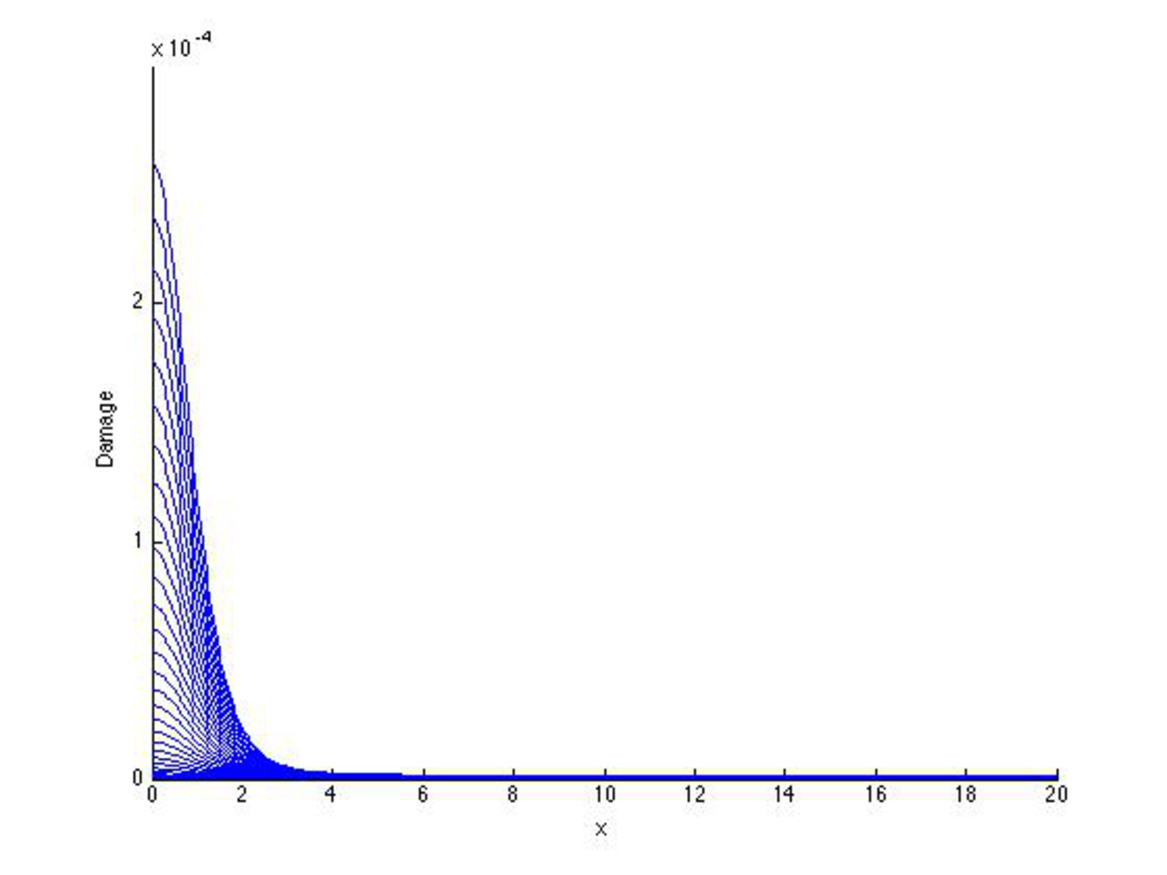
\includegraphics[scale=0.36]{Pages/Damage_Jessica.pdf}
\end{center}
\end{frame}

\begin{frame}
\frametitle{Conclusions}
\begin{itemize}
\item{The simplified model gives results very comparable to those of the more complex model and allows direct analysis}
\item{Agreement between the two models gives us confidence in both}
\item{New damage model has firmed theoretical foundation and is easy to implement}
\item{We have confidence that a more complete analysis is now possible given more time}
\end{itemize}
\end{frame}

\begin{frame}
\centerline{\large{Thanks for your attention!}}
\end{frame}

\end{document}
